% APNs connection sequence through mitmdump on the capture access point (full text width).
% Build: pdflatex fig_sequence.tex  (vector PDF)
% Coordinates in mm, y increasing DOWNWARDS.
\documentclass[tikz,border=2pt]{standalone}
\usepackage[scaled]{helvet}
\renewcommand{\familydefault}{\sfdefault}
\usepackage[T1]{fontenc}
\usetikzlibrary{arrows.meta}

\definecolor{cTealF}{HTML}{DDF1EE}   \definecolor{cTealS}{HTML}{1D8C7B}
\definecolor{cBlueF}{HTML}{DCEAF9}   \definecolor{cBlueS}{HTML}{2F6DB5}
\definecolor{cAmbF}{HTML}{FBEBCB}    \definecolor{cAmbS}{HTML}{B8781A}
\definecolor{cGrayF}{HTML}{F1F1EF}   \definecolor{cGrayS}{HTML}{8A8A85}
\definecolor{cRed}{HTML}{B3261E}

\begin{document}
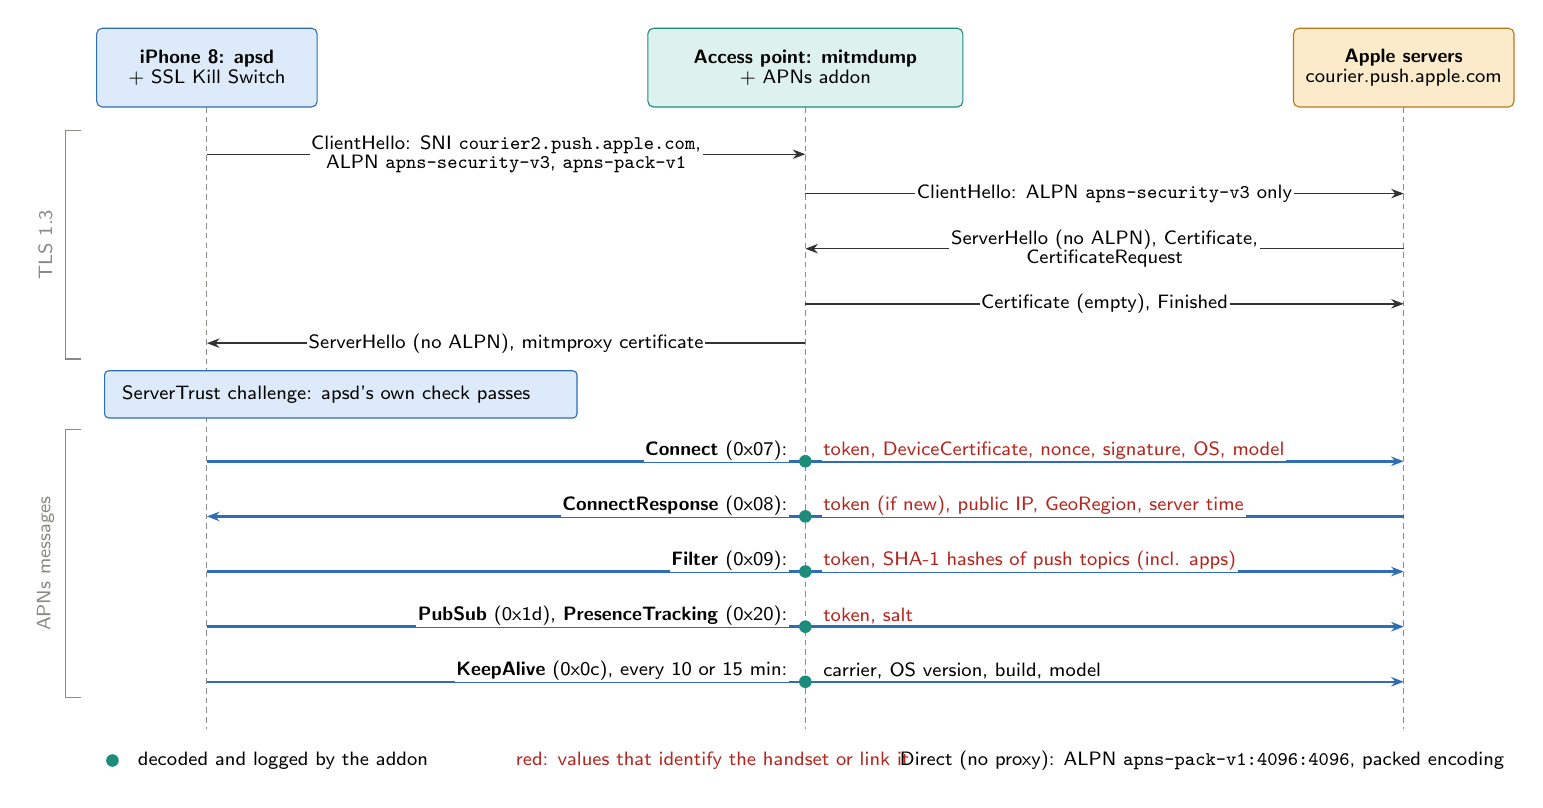
\begin{tikzpicture}[x=1mm,y=-1mm,
  msg/.style={-{Stealth[length=1.6mm,width=1.2mm]},line width=0.5pt,draw=black!80},
  app/.style={-{Stealth[length=1.6mm,width=1.2mm]},line width=0.9pt,draw=cBlueS},
  life/.style={draw=cGrayS,line width=0.4pt,dash pattern=on 2pt off 1.5pt},
  lab/.style={font=\scriptsize,inner sep=0.6pt,fill=white},
  idl/.style={font=\scriptsize,inner sep=0.6pt,fill=white,text=cRed},
  dot/.style={circle,fill=cTealS,inner sep=0pt,minimum size=1.6mm}]

% lane x positions
\def\A{14} \def\M{90} \def\C{166}

% ---- lane headers ---------------------------------------------------------
\draw[fill=cBlueF,draw=cBlueS,rounded corners=2pt] (\A-14,0) rectangle (\A+14,10);
\node[font=\scriptsize\bfseries,align=center] at (\A,5) {iPhone 8: apsd\\[-1pt]\mdseries + SSL Kill Switch};
\draw[fill=cTealF,draw=cTealS,rounded corners=2pt] (\M-20,0) rectangle (\M+20,10);
\node[font=\scriptsize\bfseries,align=center] at (\M,5) {Access point: mitmdump\\[-1pt]\mdseries + APNs addon};
\draw[fill=cAmbF,draw=cAmbS,rounded corners=2pt] (\C-14,0) rectangle (\C+14,10);
\node[font=\scriptsize\bfseries,align=center] at (\C,5) {Apple servers\\[-1pt]\mdseries courier.push.apple.com};

\draw[life] (\A,10) -- (\A,89);
\draw[life] (\M,10) -- (\M,89);
\draw[life] (\C,10) -- (\C,89);

% everything below is drawn 15 mm higher (the configuration-bag fetch and the TCP set-up are not shown)
\begin{scope}[yshift=15mm]
% ---- TLS ----------------------------------------------------------------------

\draw[msg] (\A,31) -- (\M,31) node[lab,midway,align=center] {ClientHello: SNI \texttt{courier2.push.apple.com},\\[-1pt] ALPN \texttt{apns-security-v3}, \texttt{apns-pack-v1}};
\draw[msg] (\M,36) -- (\C,36) node[lab,midway] {ClientHello: ALPN \texttt{apns-security-v3} only};
\draw[msg] (\C,43) -- (\M,43) node[lab,midway,align=center] {ServerHello (no ALPN), Certificate,\\[-1pt] CertificateRequest};
\draw[msg] (\M,50) -- (\C,50) node[lab,midway] {Certificate (empty), Finished};
\draw[msg] (\M,55) -- (\A,55) node[lab,midway] {ServerHello (no ALPN), mitmproxy certificate};

\draw[fill=cBlueF,draw=cBlueS,rounded corners=1.5pt] (\A-13,58.5) rectangle (\A+47,64.5);
\node[font=\scriptsize,anchor=west] at (\A-12,61.5) {ServerTrust challenge: apsd's own check passes};

% ---- APNs messages (serial framing), decoded by the addon ---------------------
\foreach \y/\dir in {70/1,77/-1,84/1,91/1,98/1} {
  \ifnum\dir=1 \draw[app] (\A,\y) -- (\C,\y); \else \draw[app] (\C,\y) -- (\A,\y); \fi
  \node[dot] at (\M,\y) {};
}
\node[lab,anchor=east] at (\M-2,68.6) {\textbf{Connect} (0x07):};
\node[idl,anchor=west] at (\M+2,68.6) {token, DeviceCertificate, nonce, signature, OS, model};
\node[lab,anchor=east] at (\M-2,75.6) {\textbf{ConnectResponse} (0x08):};
\node[idl,anchor=west] at (\M+2,75.6) {token (if new), public IP, GeoRegion, server time};
\node[lab,anchor=east] at (\M-2,82.6) {\textbf{Filter} (0x09):};
\node[idl,anchor=west] at (\M+2,82.6) {token, SHA-1 hashes of push topics (incl. apps)};
\node[lab,anchor=east] at (\M-2,89.6) {\textbf{PubSub} (0x1d), \textbf{PresenceTracking} (0x20):};
\node[idl,anchor=west] at (\M+2,89.6) {token, salt};
\node[lab,anchor=east] at (\M-2,96.6) {\textbf{KeepAlive} (0x0c), every 10 or 15 min:};
\node[lab,anchor=west] at (\M+2,96.6) {carrier, OS version, build, model};

% ---- phase brackets -------------------------------------------------------------
\draw[cGrayS,line width=0.5pt] (-2,28) -- (-4,28) -- (-4,57) -- (-2,57);
\node[font=\scriptsize,rotate=90,text=cGrayS] at (-6.5,42.5) {TLS 1.3};
\draw[cGrayS,line width=0.5pt] (-2,66) -- (-4,66) -- (-4,100) -- (-2,100);
\node[font=\scriptsize,rotate=90,text=cGrayS] at (-6.5,83) {APNs messages};

% ---- legend ---------------------------------------------------------------------
\node[dot] at (2,108) {};
\node[font=\scriptsize,anchor=west] at (4,108) {decoded and logged by the addon};
\node[font=\scriptsize,anchor=west,text=cRed] at (52,108) {red: values that identify the handset or link it};
\node[font=\scriptsize,anchor=east,align=right] at (\C+14,108) {Direct (no proxy): ALPN \texttt{apns-pack-v1:4096:4096}, packed encoding};
\end{scope}
\end{tikzpicture}
\end{document}
